\section{Desarrollo teórico de la fuerza de torsión en una pala de una turbina eólica}

\subsection{Descripción de la pala del aerogenerador y sus parámetros}

En esta sección se va a describir la pala del aerogenerador y los parámetros necesarios para determinar los efectos que produce la torsión en nuestra obtención de energía. En primer lugar definición e idea general de una pala, desarrollo trigonométrico para el cálculo de la línea de cuerda,... \colorbox{orange}{RELLENAR}


Se determina que la pala de la turbina eólica es un \textbf{trapecio} cuya representación simplificada se muestra en la Figura \ref{fig:pala_simp}. \\\\


\textcolor{red}{\Large{CAMBIAR LA NOMENCLATURA DE LAS FIGURAS}}

\begin{figure}[H]
    \centering
    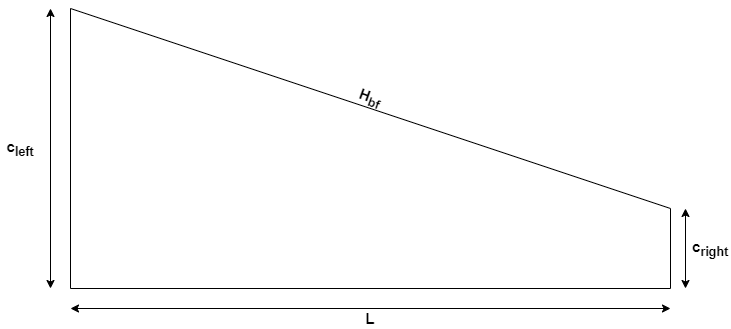
\includegraphics[width=0.7\textwidth]{images/pala simple.png}
    \caption{Representación de una pala de turbina eólica}
    \label{fig:pala_simp}
\end{figure}


Lo siguiente que debe tenerse presente es que se necesita también una representación de la pala como la que se puede observar en la Figura \ref{fig:pala_simp}. Esta está dividida en segmentos de igual largo para poder comprender el desarrollo que se realizará simulando una torsión, en la cual se girarán los segmentos un cierto ángulo los unos de los otros.

\begin{figure}[H]
    \centering
    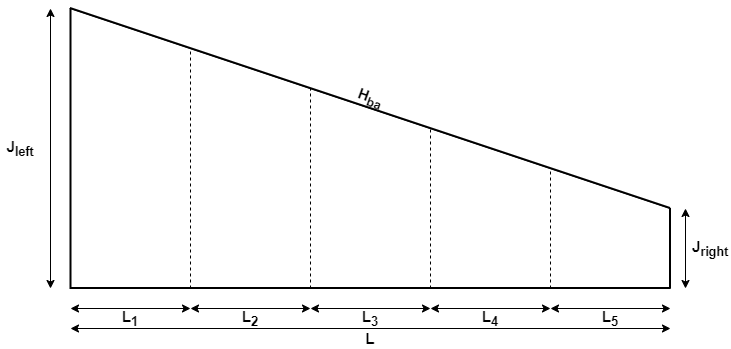
\includegraphics[width=0.7\textwidth]{images/pala simple segmentada.png}
    \caption{Representación de una pala de turbina eólica dividida en segmentos}
    \label{fig:pala_dividida}
\end{figure}

Por simplicidad, la pala se dividirá únicamente en $N$ segmentos, en este trabajo se utilizará $N=5$. Aunque se mantenga este valor durante el trabajo se asociará a una variable en caso de que se quieran hacer pruebas mediante simulación en MATLAB más adelante. \\\\
    

Se define la variable $L$ como la longitud de la pala (ver Figura \ref{fig:pala_simp}). Como puede observarse, cada uno de los segmentos de la Figura \ref{fig:pala_dividida} tendrá una longitud de segmento $L_i = \dfrac{L}{N} (m)$ donde $i \in \{1,...,N\}$.\\

Como se puede observar en la Figura \ref{fig:pala_dividida} cada segmento tiene una altura variable, esto se debe a la forma real de las palas, cuanto más cerca del buje de la turbina, mayor es el área del segmento. La altura en el centro de estos segmentos, conocida como \textit{chord line} (que se denotará como $c_i$ con $i \in \{1, ...,N\}$) o línea de cuerda, se determinará fijando los valores de la longitud de la pala $L$, la longitud del buje (que se denotará por $J_{left}$) y la longitud de la punta (que se denotará por $J_{right}$). Una vez establecidos estos valores se puede dar paso al desarrollo matemático de la pala.\\

\begin{figure}[H]
    \centering
    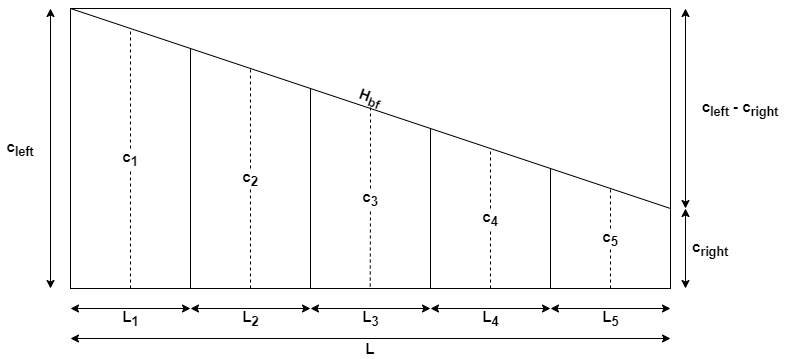
\includegraphics[width=0.9\textwidth]{images/planteo chord line.png}
    \caption{Representación parametrizada de la pala de una turbina eólica}
    
    \label{fig:pala_desarrollo_chord}
\end{figure}

Para el cálculo de la línea de cuerda se requiere la realización de un desarrollo trigonométrico. \\

En base a la Figura \ref{fig:pala_desarrollo_chord} se puede deducir que
$J_{rigth} = \dfrac{J_{left}}{D} (m)$ donde D es el factor de reducción de alto de pala y $D \in \mathbb{Q+}$. Además, se debe cumplir que $J_{left} > D$.\\

El factor reductor $D$ procede de la naturaleza del análisis y cómo se ha afrontado el estudio simplificado de una pala de aerogenerador. Si bien es cierto que se pudo realizar de una manera aún más simple haciendo que la pala fuese un rectángulo, se prefirió abordar con una forma trapezoidal. Así, los tres parámetros $J_{left}$, $J_{rigth}$ y $L$ se calculan en función del valor de $D$. Esto permite hacer los cálculos con una relación entre la longitud del buje $J_{left}$ y de la punta $J_{right}$ de las palas de la turbina eólica, esto además permite que el problema sea más general. \\

Se define el valor de la hipotenusa del borde de arrastre $H_{ba}$ mediante el Teorema de Pitágoras, ya que se trata de un triángulo rectángulo (en azul en la Figura \ref{fig:pala_calculo_phi}). Así, se tiene:
\begin{equation}
H_{ba} = \sqrt{(J_{left} - J_{right})^{2} + L^{2}}
\label{def_hipotenusa_pala}
\end{equation}


\begin{figure}[H]
    \centering
    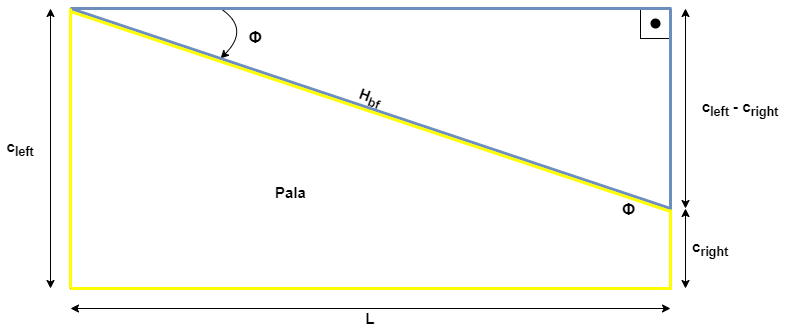
\includegraphics[width=0.9\textwidth]{images/triangulo sacar phi.drawio.png}
    \caption{Pala de la turbina en amarillo y triángulo usado para el cálculo de $\Phi$ en azul}
    
    \label{fig:pala_calculo_phi}
\end{figure}

A continuación, se debe obtener el ángulo de la línea del borde de arrastre de la pala de la turbina eólica $\Phi$, para así conocer cómo decrece el valor de $H_{ba}$.
En base a la Figura \ref{fig:pala_calculo_phi} se puede calcular de tres formas distintas mediante la trigonometría el valor del ángulo $\Phi$:
\begin{equation}
 \Phi = \arcsin{\left(\dfrac{c_{left} - c_{right}}{H_{ba}}\right)} (^{\circ})
\label{def_angulo_phi_1}
\end{equation}

\begin{equation}
 \Phi = \arccos{\left(\dfrac{L}{H_{ba}}\right)} (^{\circ})
\label{def_angulo_phi_2}
\end{equation}

\begin{equation}
 \Phi = \arctan{\left(\dfrac{\sin{\left(\dfrac{c_{left} - c_{right}}{H_{ba}}\right)}}{\cos{\left(\dfrac{L}{H_{ba}}\right)}}\right)} (^{\circ}) 
\label{def_angulo_phi_3}
\end{equation}

\colorbox{orange}{HACERLO CON TALES}


\\

% Para calcular las \textit{líneas de cuerda} $c$, se aíslan los trapecios más pequeños de los que se han obtenido todos los datos menos el valor de su base menor que se tendrá que calcular, siendo este equivalente a $c$.\\

% \begin{equation}
% Variables necesarias para el cálculo de las líneas de cuerda.

% $$ altura_i = \dfrac{(2i - 1) \cdot L}{2N}$$
% $$ diagonal_i = \dfrac{(2i - 1) \cdot H_{bf}}{2N}$$

% Donde,
% \centering
% $altura_i$ := Longitud de la pala fragmentada para el cálculo de la línea de cuerda y $diagonal_i$ := Longitud de la hipotenusa del borde de fuga fragmentada para el cálculo de la línea de cuerda.
% \label{def_variables_fragmentadas}
% \end{equation}

% Por último y una vez definido todo lo necesario, se pasa al cálculo mediante el cual se obtiene el valor de todas y cada una de las $líneas \text{ } de \text{ } cuerda$ de la pala con la que se está trabajando.

% \begin{equation}
% Primero se obtiene la diferencia mediante Pitágoras entre la base mayor y la menor, definida como $x_i$, después la resta de la base mayor y esta diferencia.

% $$ x_i = \sqrt{diagonal_i^{2} - altura_i^{2}}$$

% $$ c_i = c_{left_i} - x_i $$
% \label{def_chord_line}
% \end{equation}

% La siguiente figura, ilustra el ejemplo en el que para las definiciones \ref{def_variables_fragmentadas} y \ref{def_chord_line} el valor de $i$ es igual a 3. Obteniendo así $c_3$. En verde el trapecio y en magenta el triángulo del que restamos el cateto a la base mayor del trapecio.

% \begin{figure}[H]
%     \centering
%     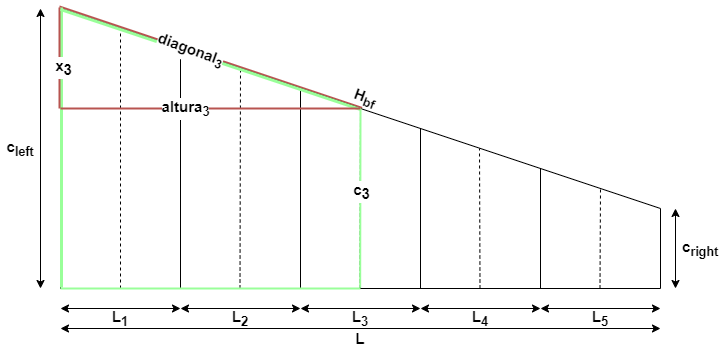
\includegraphics[width=0.9\textwidth]{images/Trapecio calculo x.png}
%     \caption{Representación gráfica del cálculo realizado en las definiciones \ref{def_variables_fragmentadas} y \ref{def_chord_line}}
% \end{figure}


% Una vez se ha obtenido el valor buscado $c_i$, se deberá definir todos los laterales de los segmentos de la pala, para así poder operar con ellos en pos de conseguir el área de cada uno de ellos. Esto ya fue desarrollado en el artículo \cite{armenta2021predictive}, pero en aquel caso fue usado para comprobar el error que suponía usar un rectángulo en vez de una pala simplificada. En este caso se parte directamente de la pala simplificada para evitar correcciones de errores mas adelante y porque el cálculo que se debe realizar con respecto a la obtención de energía no es tan profundo y complicado como en el artículo \cite{armenta2021predictive}. Además remarcar que para las deducciones y cálculos anteriores se bebió de este desarrollo.


% \begin{equation}
% En base a esta representación esquemática y mediante relaciones trigonométricas obtuvieron:
% $$ c_{left_i} = c_i + (\dfrac{L_i}{2}) \tan \varPhi$$
% $$ c_{right_i} = c_i - (\dfrac{L_i}{2}) \tan \varPhi$$
% \label{def:laterales_segmento}
% \end{equation}

% Al igual que se deduce en el artículo \cite{armenta2021predictive}, con los datos obtenidos de los laterales de cada segmento, se puede trabajar con una forma de trapecio y encontrar el área de los segmentos que se definieron en la Figura \ref{fig:pala_dividida}.\\

% Aparte, con esta definición se ve que en la Figura \ref{fig:pala_desarrollo_chord} los valores de $c_{left_i}$ y de $c_{right_i}$ que se observan, realmente serían equivalentes a $c_{left_1}$ y a $c_{right_5}$, respectivamente. Estos son definidos a priori debido a su importancia para caracterizar la pala de manera correcta y con las dimensiones que el usuario desee.

% \begin{equation}
% Se determina el área de los segmentos:
% $$ s_{i} = \dfrac{(c_{left_i} + c_{right_i})}{2N} \cdot L_i $$
% Donde,
% \centering $s_i$ := Área del segmento.
% \label{def:area_segmentos}
% \end{equation}


A continuación se supone que los segmentos están ensartados por una línea imaginaria que ayudará al estudio de la torsión mediante giros de los segmentos alrededor suya. \\

Esta línea imaginaria pasará por el centro de masas de todos los segmentos. Delineando rectas en cada segmento desde una esquina a la contraria se genera un punto en el centro del segmento en el que estas rectas se cortan, siendo este punto el llamado centro de masas. Además, si se traza una línea que una el punto central de las rectas $J_{left}$ y $J_{right}$, esta recta pasará por los centros de masa de cada uno de los segmentos.\\

Cuando se ha obtenido esta recta imaginaria, se puede determinar lo que se denotará como $brazo$ que se corresponde con la longitud desde el punto central del buje $J_{left}$ hasta la línea de cuerda $c_{i}$ del segmento $i$, siendo este punto además el centro de masas del segmento $i$.


    \begin{figure}[H]
    \centering
    \includegraphics[width=1\textwidth]{images/explicación brazo.png}
    \caption{Representación de los brazos de la pala}
    \label{fig:exp_brazo}
    
\end{figure}

El brazo viene definido por la resta de las mitades de los lados de la pala. Una vez se tiene la recta que pasa por los centros de masa se determina el valor de cada uno de los brazos.
\begin{equation}
cateto \text{ } buje = \dfrac{J_{left}}{2} - \dfrac{J_{right}}{2}
\end{equation}
\begin{equation}
R \text{ } brazo = \sqrt{cateto \text{ } buje^{2} + L^{2}}
\end{equation}
\begin{equation}
brazo_i = \dfrac{(2i -1) \cdot R \text{ } brazo}{2N}
\end{equation}
Donde, $cateto \text{ } buje$ := Medida de buje o $J_{left}$ reducida para su utilización en la obtención del brazo, $R \text{ } brazo$ := Recta completa del brazo antes de dividirla dependiendo del segmento y $brazo_i$ := Distancia entre el centro de $J_{Left}$ y el centro de masas del segmento correspondiente.

\subsection{Análisis del volumen de la pala}
\label{section:volumen_pala}

Cuando ya se ha definido la geometría de dos dimensiones de la pala del aerogenerador se puede añadir una nueva dimensión para que el análisis sea aún mas completo. Si se limitara a las dos dimensiones, las simplificación sería tal, que se perdería criterio a la hora de analizar los datos obtenidos.


    \begin{figure}[H]
    \centering
    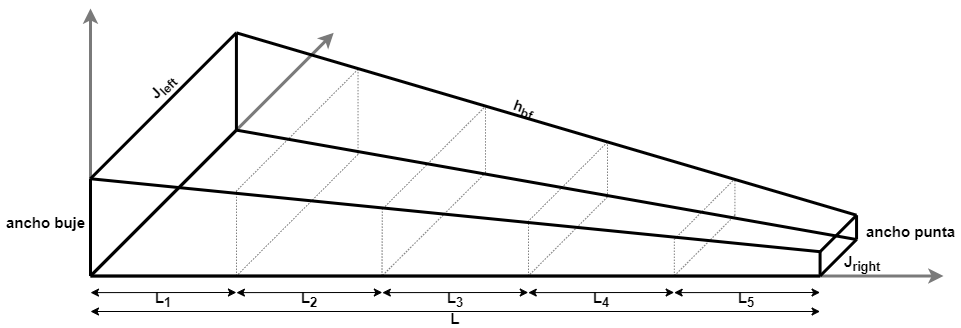
\includegraphics[width=1\textwidth]{images/pala 3d segmentada enorme.png}
    \caption{Representación gráfica de la pala segmentada en 3 dimensiones}
    \label{fig:analisis_volumen}
    
\end{figure}



Mediante la observación de la figura \ref{fig:analisis_volumen} se puede averiguar lo siguiente: \\\\\\\\

\colorbox{Orange}{ \Huge Aquí va un desarrollo con otra figura, la del ancho}

\begin{equation}
Aplicando el desarrollo explicado justo encima:
$$ recta \text{ } decrecimiento_i = \dfrac{( i \cdot \sqrt{L^2 + (ancho \text{ } punta - ancho \text{ } buje)^2)}}{N}$$
 
$$ancho \text{ } buje, ancho  \text{ } punta \in \mathbb{Q+}$$
$$ ancho \text{ } buje > ancho \text{ } punta $$

Donde,
\centering $recta \text{ } decrecimiento_i $ := línea de disminución de la parte superior ancho de la pala dividida para cada segmento,  $ancho \text{ } punta$ := amplitud de la pala del aerogenerador en la zona más estrecha o punta y $ancho \text{ } buje$ := amplitud de la pala del aerogenerador en la zona más ancha o buje.
\label{def:ancho_buje_punta}
\end{equation}


Tal y como se presentó en la Figura \ref{fig:pala_calculo_phi}, la variable $x_i$ sirvió de apoyo para calcular las reducciones de tamaño de las líneas de cuerda al ir restando el resultado a la variable $c_left_{i}$. Esto mismo ocurre para el ancho de la pala mediante el uso de la Definición \ref{def:ancho_buje_punta} y el Teorema de Pitágoras. En esta ocasión además, se necesitará una segunda variable que se explicará mas adelante, debido a la forma en tres dimensiones de la pala. 



\begin{equation}
Las variables de apoyo son las siguientes:
$$ z_i = \sqrt{ recta \text{ } decrecimiento_i^2 - (L_i \cdot i )^2 }$$
$$ b_i =  \left\{\begin{matrix}
0 \hspace{33pt} Sí \hspace{7pt} i = 1\\ 
z_i  \hspace{30pt} Sí \hspace{7pt}  i > 1
\end{matrix}\right$$
Donde,
$z_i$ := variable de apoyo para el cálculo del área de las secciones trapezoides correspondientes al corte de los segmentos, en este caso de las bases menores,  $b_i$ := segunda variable de apoyo pero en este caso sirve para las bases mayores.
\centering 
\label{def:variables_apoyo}
\end{equation}

¿Por qué en las descripciones se habla de bases mayores y menores? Es sencillo, debido a la geometría de la pala, como se puede vislumbrar en la Figura \ref{fig:analisis_volumen} y los cortes hechos para dividir la pala en $N$ segmentos crean una forma de tronco de pirámide trapezoidal. Tanto si se divide como si no, el volumen se analizará exactamente de la misma manera, mediante las fórmulas deducidas y posteriormente expandidas a otros casos de uso como el nuestro que se encuentran en el \textit{Moscow Mathematical Papyrus} \cite{gunn1929four}.


\begin{equation}
Se obtiene el ancho de las bases de los troncos trapezoidales y en consecuencia se calculan las áreas de las bases:
$$ ancho \text{ } bases \text{ } menores_i = ancho \text{ } buje - z_i $$
$$ ancho \text{ } bases \text{ } mayores_i = ancho \text{ } buje - b_i $$

$$ area \text{ } bases \text{ } menores_i = ancho \text{ } bases \text{ } menores_i \cdot c_{right}_i $$ 
$$ area \text{ } bases \text{ } mayores_i = ancho \text{ } bases \text{ } mayores_i \cdot c_{left}_i $$
Donde,
\centering $ancho \text{ } bases \text{ } mayores_i$ := Ancho de las bases trapezoidales de mayor tamaño con las que se calculará el volumen del tronco o frustum de cada uno de los segmentos,  $ancho \text{ } bases \text{ } menores_i$ := Ancho de las bases trapezoidales de menor tamaño con las que se calculará el volumen del tronco o frustum de cada uno de los segmentos, $ area \text{ } base \text{ } mayor_i $ := zonas trapezoidales que sirven de base mayor para el cálculo del frustum de cada segmento y $ area \text{ } base \text{ } menorr_i $ := zonas trapezoidales que sirven de base menor para el cálculo del frustum de cada segmento.
\label{def:area_bases}
\end{equation}


Con todo lo necesario para el cálculo del volumen de la pala del aerogenerador se procede a ello. Añadir que se va a realizar de dos maneras; completo y segmentado. El segmentado es necesario debido al desarrollo que se ha ido realizando y que se va a seguir durante todo el trabajo y el completo lo usamos para comparación y demostrar que segmentado o no, es correcto.


\begin{equation}
El volumen de nuestra pala de una turbina eólica completa y simplificada es:
    \begin{align*}
        volumen \text{ } frustum_i = & \dfrac{L_i}{3} \cdot (area \text{ } bases \text{ } mayores_i + area \text{ } bases \text{ } menores_i + \\
        & \sqrt{area \text{ } bases \text{ } mayores_i \cdot area \text{ } bases \text{ } menores_i})
    \end{align*}
$$ volumen \text{ } frustum_{total} = \sum_{i}^{N}volumen \text{ } frustum_i  $$

$$ area \text{ } base_{punta} = ancho \text{ } punta * J_{right} $$
$$ area \text{ } base_{buje} = ancho \text{ } buje * J_{left} $$
$$ volumen \text{ } frustum_{completo} = \dfrac{L}{3} \cdot ( area \text{ } base_{punta} + area \text{ } base_{buje} + \sqrt{area \text{ } base_{punta} \cdot area \text{ } base_{buje}} ) $$


Donde,
\centering $ volumen \text{ } frustum_i $ := tamaño de cada uno de los segmentos del tronco de pirámide de la pala del aerogenerador, $ volumen \text{ } frustum_{total} $ := tamaño absoluto de la pala del aerogenerador, $area \text{ } base_{punta}$ := zona trapezoidal de mayor tamaño usada para el cálculo del volumen del frustum, $area \text{ } base_{punta}$ := zona trapezoidal de menor tamaño usada para el cálculo del volumen del frustum y $ volumen \text{ } frustum_{completo} $ := tamaño integro de la pala del aerogenerador.
\label{def:volumen_tronco_frustum}
\end{equation}


Teniendo los cálculos del volumen de la pala del aerogenerador se puede pasar a lo siguiente, estudiar los efectos que producen las especificaciones y simplificaciones que se han realizado para la obtención de energía.


\subsection{Estudio del torque sin ángulo de cabeceo}
\label{section:torque_pala_horizontal}
En este apartado y tomando la pala con una forma real y no una simplificada como con la que se trabaja, se puede observar un primer caso en el cual ya se produce un giro de las palas del aerogenerador. \\

Esta situación es en la cual no se presenta cabeceo, es decir, el viento tiene un ángulo de ataque paralelo para con la pala de la turbina eólica. \\

Pero, al tomar una pala real, la cual está más redondeada por la parte superior y teniendo mayor volumen que la parte inferior. Por ello mediante el principio Bernoulli, se ve que esta parte superior presenta un mayor recorrido que la inferior y con ello una velocidad de viento mayor por tanto una menor presión. \\

Este efecto produce un gradiente de presión y por ello una fuerza de sustentación. Todo ello por la no simetría de las palas del aerogenerador. \\

Debido a este fenómeno, se produce una situación de estudio poco favorable. Es por esto y otros motivos por lo cual se trabaja con una pala simplificada que ayuda al trabajo y posteriores cálculos y por lo que los siguientes apartados son aquellos con mayor peso técnico y explicativo. \\





















\subsection{Estudio del torque con ángulo de cabeceo}
\label{section:torque_giro_inicial}

Se han presentado algunos de los conceptos básicos, ahora se introduce el ángulo $ \theta_1 $, que es la constante definida como el \textit{ángulo de cabeceo} que sufrirán todos y cada uno de los segmentos que son paralelos al plano horizontal, desde el cual se presenta el viento que incidirá en nuestra pala.\\


En esta primera sección se estudiará qué ocurre en término de fuerzas, torque y momento cuando se gira toda nuestra pala únicamente el ángulo de cabeceo $ \theta_1 $. \\


Es cierto que se podría no girar la pala este ángulo $ \theta_1 $, pero por comodidad de cálculo y para establecer un ángulo de ataque del viento paralelo a la horizontal se realizará de esta manera.\\


Al haber inclinado todos los segmentos un ángulo $ \theta_1 $ se genera la situación en la que el viento incide en el centro del segmento con el mismo ángulo con el que se inclina la pala. \\

    \textbf{}
    \begin{figure}[H]
    \centering
    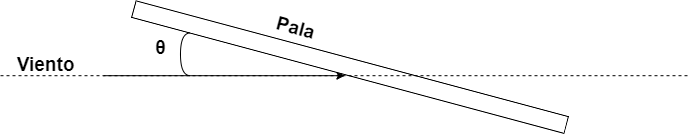
\includegraphics[width=0.8\textwidth]{images/dibujo angulo ataque.drawio.png}
    \caption{Ángulo de ataque del viento con respecto a la pala}
    
    \label{fig:dibujo_angulo_ataque}
\end{figure}

La fuerza del viento que incide en la pala se puede descomponer en 2, la tangencial y la normal. \\

    \textbf{}
    \begin{figure}[H]
    \centering
    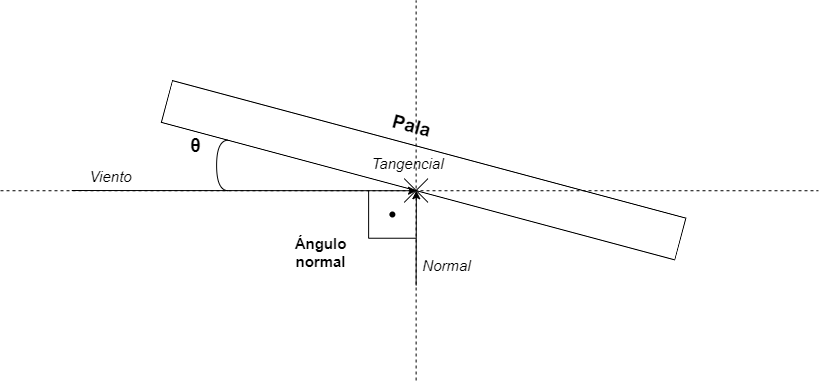
\includegraphics[width=1\textwidth]{images/dibujo fuerzas.drawio.png}
    \caption{Descomposición de vectores de fuerzas}
    
    \label{fig:dibujo_fuerzas}
\end{figure}


Como se puede ver en la figura \ref{fig:dibujo_fuerzas} el vector fuerza normal es perpendicular al ángulo de ataque del viento, mientras que el vector fuerza tangencial recorre de manera paralela la línea central de la pala.

%  \begin{equation}
%  La fuerza normal genera un ángulo definido por:
%  $$ n = \dfrac{\pi}{2} - \theta_1 $$
%  Donde,
%  \centering $n$ := ángulo normal.
%  \end{equation}

 \begin{equation}
 La fuerza normal viene definida por la siguiente expresión:
  $$ f \text{ } normal_i = F \text{ } viento_i \cdot \sin{\theta_1}$$
Donde,
\centering $F \text{ } viento$ := Fuerza generada por el viento en cada segmento de la pala y $f \text{ } normal$ := Fuerza perpendicular al viento, generada por el choque de este con la pala de la turbina eólica.
 \label{def:fuerza_normal}
 \end{equation}
 
  La componente paralela a la pala, que se ha definido como tangencial se obviará debido a que no genera momento de torsión o torque. 
  
  \begin{equation}
El momento de giro o torque se define como:
 $$ torque_0 = f \text{ } normal_i \times brazo$$
Donde,
\centering $torque_0$ := Momento de fuerza de giro solo con ángulo de cabeceo.
  \label{def:torque_inicial}
 \end{equation}
 

 En la Definición \ref{def:torque_inicial} se encuentra un producto vectorial entre la $fuerza  \text{ }perpendicular \text{ } o \text{ } normal$ y el $brazo$. Pero estas dos variables son perpendiculares la una a la otra. Esto se puede ver ya que $brazo$ es completamente paralelo a la $fuerza \text{ } tangencial$. Esto demuestra la perpendicularidad y hace que la Definición \ref{def:torque_inicial} que contenía un producto vectorial de dos parámetros perpendiculares sea definitivamente un producto algebraico, dando lugar a:
 
 
  \begin{equation}
  El torque termina siendo un producto algebraico.
 $$ torque_{0_i} = f \text{ } normal_i \cdot brazo_i$$
 \label{def:torque_algebraico_inicial}
 \end{equation}
 
 
 \begin{equation}
 La suma de los torques con un ángulo de cabeceo se conoce como torque global.
 $$ torque \text{ } global_0 \text{ } = \sum_{i=1}^{N} torque_0_{i} $$
\label{def:torque_global}
\end{equation}
 
 \\\\Ahora se introduce otro concepto, se trata de la \textit{fuerza del viento}. Gracias a este parámetro, se podrá conocer la fuerza normal que se está produciendo en todo el rotor mediante la definición \ref{def:fuerza_normal}.
 
 
 \begin{equation}
 La fuerza del viento para el rotor completo:
 
 $$ F \text{ } viento_i = \dfrac{1}{2} \text{ } \rho \cdot area \text{ } rotor \cdot u^2 \cdot coeficiente \text{ } sustentación$$
 $$ area \text{ } rotor = \dfrac{\pi}{4} \cdot diametro \text{ } rotor $$
 $$ diametro \text{ } rotor = 2 \cdot L^2 $$
Donde,
 \centering  $\rho = 1.225 \text{ } \dfrac{Kg}{m^3}$ y $u$ := velocidad del viento.
 \label{def:fuerza_viento_inicial}
 \end{equation}
 
\vspace{15pt} Entendido esto, ya se podría pasar a calcular el valor del $torque \text{ } global_i$.
 
 
 
 
 
 
 
 
 
 
 
 
 \subsection{Estudio del torque con ángulo de cabeceo y torsión de la pala}
\label{section:torque_giro_torsion}

La única diferencia entre este apartado y el anterior es el ángulo de giro de los segmentos. En la sección \ref{section:torque_giro_inicial} se vió como todos los segmentos giraban únicamente un determinado \textit{ángulo de cabeceo}, pero ahora y en pos del estudio de la torsión, el ángulo que se girarán vendrá dado por la siguiente definición: 


\begin{equation}
Dados el ángulo inicial de giro $\theta_1 $ y una variación de giro constante (o no) $\Delta_\theta$ se define el ángulo de torsión de cada segmento como:
$$\theta_i = \theta_{i-1} + \Delta_\theta$$ 
Donde,
\centering $i \in segmento \wedge (i > 1)$

\label{def:theta_cte}
\end{equation}


\begin{equation}
Como se menciona, la variación $\Delta_\theta$ puede que no sea constante por conveniencia a la hora de calcular resultados futuros, por ello la definición también puede darse de la siguiente forma:
$$\theta_i = \theta_{i-1} + \Delta_{\theta_{i}}$$ 
Donde,
\centering $i \in segmento \wedge (i > 1)$
\label{def:theta_nocte}
\end{equation}


Esto provoca que algunas de las definiciones anteriores se vean alteradas por el cambio que presenta la variable $\theta_i$.\\

% \begin{equation}
%  La fuerza normal genera un ángulo de:
%  $$ n_i = \dfrac{\pi}{2} - \theta_i $$
 
%  Donde,
%  \centering $i \in segmento$
%  \end{equation}

 \begin{equation}
  Su fuerza se define como:
  $$ f \text{ } normal_i = F \text{ } viento_i \cdot \sin{\theta_i}$$
  \label{def:fuerza_normal_torsion}
 \end{equation}

El resto de fórmulas no varían debido a que no dependen del ángulo $\theta_i$, tienen exactamente la misma definición. Pero en el caso del \textit{torque global} si que cambia, ya que la suma de torques nos aportará un conjunto de valores diferentes y que servirán como estudio. \\\\

  \begin{equation}
  El torque termina siendo un producto algebraico.
 $$ torque_{1_i} = f \text{ } normal_i \cdot brazo_i \cdot \cos{\Delta_{\theta_{i}}}$$
 \label{def:torque_algebraico_torsion}
 \end{equation}
 
 En la definición \ref{def:torque_algebraico_torsion} se introduce un nuevo término, $ \cos{\Delta_{\theta_{i}}} $ este aunque pueda presentar únicamente una pequeña variación en el valor del torque es imprescindible, ya que no incluirlo haría que no se estuviera realizando correctamente el cálculo. Este coseno representa por así llamarlo el área efectiva donde se está aplicando la $ f \text{ } normal $, es decir, el área de la totalidad del segmento de la pala que se vería de esta si se observara con una vista de pájaro como en la Figura \ref{fig:exp_brazo}. \\

\begin{equation}
 La suma de los torques con un giro inicial se conoce como torque global.
 $$ torque \text{ } global_1 \text{ } = \sum_{i=1}^{N} torque_{1_i} $$
Donde,
\centering $torque \text{ } global_1$ := Suma de torque de los N segmentos.
 \label{def:torque_global_1}
\end{equation}






















\subsubsection{Cálculo de la potencia del sistema}
\label{section:pot_sistema}
 
 Una vez se tiene todo lo necesario para el cálculo del torque, se puede pasar al siguiente escalón que sería la potencia. Esta es una unidad de medida que permitirá conocer si el estudio que se está realizando está siendo fructífero, cuanta mayor cantidad de energía se genere, mejor, aunque existe un límite directamente relacionado con las limitaciones técnicas y físicas que presentan las turbinas eólicas. \\
 
  \begin{equation}
 La potencia del sistema con un ángulo de cabeceo se define como:
 $$ potencia \text{ } global_0 = torque \text{ } global_0 \cdot \Omega $$ 
 
 Donde,
  \centering $\Omega$ := velocidad de giro o angular de la pala y $potencia \text{ } global_0$ := energía del sistema unicamente con un cierto ángulo de cabeceo.
 \label{def:potencia_giro_inicial}
 \end{equation}
 
   \begin{equation}
 La potencia del sistema con un giro inicial y torsión se define como:
 $$ potencia \text{ } global_1 = torque \text{ } global_1 \cdot \Omega $$ 
 
 Donde,
 \centering $potencia \text{ } global_1$ := Energía del sistema con un cierto ángulo de cabeceo y segmentos torsionados.
 \label{def:potencia_giro_segmentos}
 \end{equation}
 
 
Las unidades que se buscan serían, la potencia en $W$ ($Watts$) o $\dfrac{J}{s}$ ($\dfrac{Julio}{segundo}$) porque el torque es en $\dfrac{N}{m}$ ($\dfrac{Newton}{metro}$) o $J$ y $\Omega$ en $\dfrac{1}{s}$ o $s^{-1}$. Si todo el desarrollo arriba es correcto, en primera instancia las unidades deberían ser correctas, en caso de no serlo los valores finales a los que se está intentando llegar serían muy dispares. \\

 
 Como se puede observar, se calculó dos veces la potencia, una por cada apartado estudiado. La definición \ref{def:potencia_giro_inicial} corresponde a la sección \ref{section:torque_giro_inicial} que se referencia con un $0$ ya que es la situación inicial y más básica. Mientras que la definición \ref{def:potencia_giro_segmentos} corresponde a la sección \ref{section:torque_giro_torsion} que se ha referenciado con un $1$ ya que nace de la primera.
 
\subsection{Momento de inercia general de los segmentos de la pala}

Para poder llegar a la $\Omega$ que se usa en la Sección \ref{section:pot_sistema} es necesario pasar por dos desarrollos siendo este el primero y relacionado con el momento de inercia.\\

Pero, ¿qué es el momento de inercia? Según el Libro de Eugen Goldstein \cite[.~269]{goldstein1987mecanica}, el $momento \text{ } de \text{ } inercia$ respecto a un eje se define diciendo que es la suma, extendida a todas las partículas del cuerpo, del producto de la masa de cada partícula por el cuadrado de su distancia al eje.\\


La geometría del cuerpo libre que está realizando la rotación es crucial, es por ello que dependiendo de esta, el cálculo del momento de inercia variará. En el libro \textbf{Machinery’s
Handbook}, se pueden observar algunos de los momentos de inercia del área de algunos objetos, en concreto triangulares y otros poligonales, estando dentro de estos últimos el de un trapecio y como se pudo observar anteriormente en concreto en la Figura \ref{fig:pala_dividida} cuando se divide la pala en segmentos, cada uno de estos también pasa a ser un trapecio.\\

El hecho de que cada segmento sea a su vez un trapecio es lo que hace que se escoja la fórmula del momento de inercia del área de un trapecio presentada en este libro \cite[p.~242]{oberg2012machinery}. \\

Pero antes de pasar a trabajar con esta fórmula y su desarrollo, se debe entender la física detrás del problema que se tiene con la pala. El momento de inercia generalmente se calcula mediante el conocimiento de la posición del centro de masa de la figura que se está estudiando, suele usarse para figuras complejas que son conformadas por otras mas simples, pero en nuestro caso solo se trata de una figura simple. Pero estas figuras que giran en base a un eje, como menciona la definición del momento de inercia, no siempre lo hacen con respecto al eje perpendicular que atraviesa el centro de masa, en ocasiones el eje de giro se encuentra fuera de la figura, es donde entra el $Teorema \text{ } de \text{ } Huygens-Steiner$ o $Teorema \text{ } del \text{ } eje \text{ } paralelo$ \textcolor{red}{no encuentro una buena referencia para este teorema, supuestamente viene en Introduction to Theoretical Physics, de 1928, pero no encuentro este libro} \\

Este teorema establece que se puede calcular el momento de inercia de un cuerpo rígido en cualquier eje paralelo al que pasa atravesando la figura por el centro de masas. Para esto, es necesario conocer la distancia perpendicular entre los ejes paralelos, que se definió anteriormente como $brazo$ y la masa del cuerpo, aunque en nuestro caso será la masa de cada segmento. \\\\\\


 \begin{Teorema}
El teorema de Huygens-Steiner establece lo siguiente:

$$I = I_{cm} + m \cdot D^2$$

 Donde, $I$ := momento de inercia general, $I_{cm}$ := momento de inercia en el centro de masas de un cuerpo rígido, $m$ := masa del cuerpo rígido y $D$ := distancia perpendicular entre los ejes paralelos.
 \centering 
 \label{theo:Huygens-Steiner}
 \end{Teorema}

Para poder llegar a calcular el $momento \text{ } de \text{ } inercia \text{ } general$ o $I$ primero se debe obtener el $I_{cm}$ pero, aun no se ha definido como obtener este.\\

En este apartado se comenta que en el libro \textbf{Machinery’s Handbook} aparecen el momento de inercia de un área trapezoidal:

 \begin{equation}
El momento de inercia viene dado por la siguiente definición:

 $$ I_{area} = \dfrac{ L_{i}^3 \cdot (c_{right}^2 + 4 c_{right} \cdot c_{left} + c_{left}^2)}{ 36 (c_{right} + c_{left})} $$ 
 
 Donde, $I_{area}$ := momento de inercia de área de una figura de un espesor mínimo para centrar su cálculo en la forma.
 \centering 
 \label{def:momento_inercia_area}
 \end{equation}
 
 El "problema" de la Definición \ref{def:momento_inercia_area} es que no se presenta en las unidades que presenta de manera general el momento de inercia, para ello se debe multiplicar este por la \textbf{densidad superficial} de la pala del aerogenerador y así obtener $Kg \cdot m^2$ con los que es posible trabajar y enlazar con el Teorema \ref{theo:Huygens-Steiner} \\

En el cálculo de la \textbf{densidad superficial} son necesarios dos términos que aún no se han acuñado en este trabajo, la masa y la superficie de una pala. Es cierto que se ha calculado la superficie de los segmentos en la Definición \ref{def:area_segmentos}, ahora solo queda sumarlos.

 \begin{equation}
La superficie de la pala viene definida por la siguiente expresión, teniendo en cuenta definiciones anteriores:

$$ Superficie \text{ } pala = \sum_{i}^{N}s_i  $$

 Donde, $ Superficie \text{ } pala $ := área de la pala del rotor
 \label{def:superficie_pala}
 \end{equation}

Antes de continuar y definir la masa de la pala, se deben conocer los materiales de los que posiblemente esté compuesta, para este trabajo solo se han tenido en cuenta 3 de los más usados.

 \begin{equation}
Los rangos de densidades de materiales usadas son los siguientes:

$$ densidad \text{ } pala =  \left\{\begin{matrix}
CFRP = 1500-2000 \text{ } \dfrac{Kg}{m^3} \cite{MOHAMMED201969}\\\\
GFRP = 910-1200 \text{ } \dfrac{Kg}{m^3}  \cite{Ephraim2015}\\\\
GF \text{ } Epoxy = 1159-1186 \text{ } \dfrac{Kg}{m^3} \cite{Tewari2011}
\end{matrix}\right$$

%$$ CFRP = 1500-2000 \text{ } \dfrac{Kg}{m^3} \cite{MOHAMMED201969} $$ 
%$$ GFRP = 910-1200 \text{ } \dfrac{Kg}{m^3}  \cite{Ephraim2015}$$
%$$ GF \text{ } Epoxy = 1159-1186 \text{ } \dfrac{Kg}{m^3} \cite{Tewari2011} $$

 Donde, $ densidad \text{ } pala $ := densidad de los materiales de los que posiblemente esté compuesta la pala, $ CFRP $ := Carbon fiber reinforced polymer o en castellano; polímero reforzado con fibra de carbono, $ GFRP $ := Glass fiber reinforced polymer o en castellano; polímero reforzado con fibra de vidrio y $GF \text{ } Epoxy $ := Glass fiber reinforced Epoxy o en castellano; Epoxy reforzado con fibra de vidrio.
 \label{def:materiales_pala}
 \end{equation}

Algo que se debe saber antes de pasar a calcular la masa de la pala, es que parte de estas es hueca. Hay estudios como \textbf{Hollow Blades for Small Wind Turbines Operating at High Altitudes} \cite{Pourrajabian2016} realizado en 2016 en el que se compara el uso de palas compactas y huecas en determinado escenario y con diferentes grosores de material. Materiales tales como $GF \text{ } Epoxy$.\\

En este trabajo, las palas serán huecas y se estima que solo un $15-20\%$ de la pala presenta alguno de los materiales que se mencionan en la Definición \ref{def:materiales_pala}. Es por ello que la expresión de la masa es algo diferente. \\

 \begin{equation}
La masa de los segmentos de una pala dada su densidad y volumen:

$$ masa \text{ } pala = densidad \text{ } pala \cdot (volumen \text{ } frustum_{total} \cdot (15-20\%) ) $$

$$ masa \text{ } segmento_i = \dfrac{s_i}{superficie \text{ } pala} \cdot masa \text{ } pala $$

 Donde, $ masa \text{ } pala $ := peso de la aleta de la turbina eólica teniendo en cuenta la porción no rellena de la misma y $ masa \text{ } segmento_i $ := peso de los segmentos de la aleta.\\
 \label{def:masa_pala}
 \end{equation}
 
 Mediante las Definiciones \ref{def:superficie_pala} y \ref{def:masa_pala} se puede pasar a calcular la $densidad \text{ } superficial$.\\
 
  \begin{equation}
La densidad superficial de una pala de aerogenerador es la siguiente:

$$ densidad \text{ } superficial = \dfrac{masa \text{ } pala}{ superficie \text{ } pala}$$

 Donde, $ densidad \text{ } superficial $ := masa de un material por unidad de superficie. \\
 \label{def:densidad_superficial}
 \end{equation}
 
 
Aplicando el Teorema \ref{theo:Huygens-Steiner} se puede proceder al cálculo del momento de inercia general o $I$, ya que como se ha ido detallando a lo largo de este apartado se tiene todo lo necesario para su definición.\\

  \begin{equation}
El momento de inercia general viene dado para este estudio mediante la siguiente definición:

$$I_{cm} = I_{area} \cdot densidad \text{ } superficial $$
$$I = I_{cm} + masa \text{ } segmento_i \cdot brazo_i^2 \hspace{7pt} \dfrac{Kg}{m^3}$$

 \label{def:momento_inercia_general}
 \end{equation}
 
Con la Definición \ref{def:momento_inercia_general} concluye el apartado y se puede avanzar al siguiente, el cual es el último con desarrollos físicos sobre el giro del rotor de un aerogenerador.
 
\subsubsection{Velocidad Angular, $\Omega$, en función de la velocidad del viento }

\textcolor{red}{apartado 3.2 del libro de wind y cosas que descargué}

Este apartado responde a las definiciones de la Sección \ref{section:pot_sistema} en las cuales se usa la variable $\Omega$. Se va a estudiar de donde procede esta, pero para adelantar acontecimientos está directamente relacionada con la energía cinética del sistema formado por el rotor de la turbina eólica.\\

Lo primero que se debe conocer es ¿qué es la velocidad angular? Para responder a esta pregunta se ha recurrido al libro \textbf{Understanding Physics}. En este se define la velocidad angular, $\Omega$, como "la componente de un vector unidimensional a lo largo del eje de rotación en relación con el sistema de coordenadas elegido para describir el movimiento" \cite[p.~303]{cummings2004understanding}.\\

Aplicando la anterior definición al sistema que se está estudiando se puede comprender lo siguiente; el rotor del aerogenerador sería el eje de rotación en base al cual giran las palas de la turbina, además el movimiento de giro es constantemente alrededor del rotor y no cambiante, se aclara esto ya que la rotación angular puede ser en base a un objeto estático o a uno orbital.\\

Una de las opciones más sencillas que se tiene para el cálculo de la \textit{velocidad angular} es mediante la aceleración angular y la relación que tiene con el \textit{torque} y con el \textit{momento de inercia general}. Pero este no era lo suficientemente preciso y no tenía en cuenta todos los aspectos posibles que sí se han tenido en cuenta mediante la cinemática. \\
 
Bien es cierto que para que el sistema se encuentre girando a una cierta \textit{velocidad angular} primero se debe producir una cierta \textit{aceleración angular} producida por el viento que encontramos en el ambiente. Después si estos dos factores junto con la turbina encuentran cierto equilibrio con el rozamiento del aire, el peso de las palas y la fuerza necesaria para moverlas, se podría llegar a mantener una velocidad de giro óptima y así extraer la mayor cantidad de energía de cada giro. Pero bien es sabido que las velocidades del viento y sobretodo en zonas marítimas, es de cierta manera irregular.\\

Pero de algún modo lo que se pretende con las turbinas es que sus velocidades sean constantes y poco variables, debido al complejo sistema de engranajes que presenta dentro y que debe ir cambiando para siempre obtener la cantidad óptima de energía que es posible obtener en relación a la velocidad de viento que se presenta delante de la turbina.\\

Ahora que se tienen los conocimientos básicos sobre la velocidad angular y lo necesario para obtenerla, se puede pasar a la definición de los términos que se van a usar para su cálculo.\\

Como se comenta en uno de los párrafos de esta sección, una de las partes fundamentales es el viento que se presenta delante de la turbina y su velocidad, es decir, la masa o flujo de aire que atravesará el disco imaginario que se establece con las dimensiones de la turbina del generador eólico. Y al querer calcular una masa, en este caso del aire se obtendrá mediante la relación del volumen frente a la turbina y la densidad del mismo, esta puede variar dependiendo de las condiciones meteorológicas, pero se han obviado.\\

    \begin{equation}
    La masa de aire con la que trabaja el rotor completo se define de la siguiente forma:
    
    $$ diametro \text{ } rotor = 2L + diametro \text{ } gondola $$
    $$ volumen \text{ } rotor = \dfrac{\pi}{4} \cdot diametro \text{ } rotor^2 \cdot J_{left} $$
    $$ Masa \text{ } aire = volumen \text{ } rotor \cdot \rho $$
    Donde, blablabla
    \centering 
    \label{def:masa_aire}
    \end{equation}





\colorbox{Orange}{Falta por incluir y explicar esto:}

     Energía cinética
    
        $e cinetica = 1/2 * M aire * U VIENTO^2$
        
    Involucramos el coeficiente de potencia con la energía cinética
    
         e cinetica aprovechada = $e cinetica * CP$
         
    Ahora necesitamos la energía cinética de rotación
    
         e cinetica rotacion =$ 1/2 * I * omega^2$

    Se compara y despeja con la energía cinética aprovechada para obtener la velocidad angular omega
    
        $omega = sqrt((CP .* M aire)./I) .* U VIENTO.'$



 \subsection{Rendimiento de las potencias}
 \label{section:rendimiento}
 
Realizada la definición de cada una de las fórmulas necesarias para el cálculo de la potencia, se pasa a la comparación de estas. La comparación de potencias nos da como resultado un rendimiento, con este seremos capaces de dictaminar si la torsión de la pala genera una variación en la potencia obtenida.
 
   \begin{equation}
El rendimiento del sistema viene definido por:
 $$ \eta = \dfrac{potencia \text{ } global_1}{potencia \text{ } global_0} $$ 
 
 Donde,
  \centering $\eta$ := eficiencia respecto a la energía obtenida en dos casos estudiados.
 \label{def:rendimiento_potencias}
 \end{equation}
 
 Una vez se ha definido el rendimiento y se calcula en base a los resultados obtenidos mediante asignación de valores a variables estándar y aplicando estos a las definiciones relacionadas, se pueden dar 3 escenarios:
 

\begin{enumerate}
    \item $\eta < 1$
        \begin{itemize}
            \item En caso de obtener un valor por debajo de 1, quiere decir que la torsión que se aplicó en el caso estudiado, ha reducido la obtención de energía con respecto al caso base. 
        \end{itemize}
    \item $\eta ~= 1$
        \begin{itemize}
            \item Si el valor obtenido es muy próximo a 1, entonces el caso base y el estudiado proporcionan valores similares de obtención de energía.
        \end{itemize}
    \item $\eta > 1$
        \begin{itemize}
            \item Este es el valor buscado y el objetivo del estudio, que una pala con torsión obtenga más energía que una sin ello.
        \end{itemize}
\end{enumerate}

Cabe recalcar que se deberán hacer numerosas pruebas con diferentes configuraciones de valores .... (SEGUIR)
 
\subsection{Primeras pruebas en MATLAB}

Desarrollado todo el fundamento teórico detrás del estudio que se está realizando y con el que se está tratando de conocer si mediante torsión de las palas de una turbina eólica se obtiene más energía, menos o la misma que si no se torsionasen, se debe avanzar y comenzar a hacer cálculos empíricos. \\

Estos cálculos y representaciones se realizarán mediante MATLAB, de la manera más ordenada y arbitraria posible. Con esto se busca la manera más simple de poder modificar las variables más sencillas que envuelven a los cálculos, para así poder cambiarlas a placer. \\

Algunas variables como, $L$ y $\Theta_1$ deben ser establecidas por el propio estudiante, dando así un mayor juego a la amplitud de resultados posibles. \\